\chapter{Contributions à l'indexation automatique par termes-clés}
\chaptermark{Contribution à l'indexation par termes-clés}
\label{chap:main-automatic_keyphrase_annotation}
  \smallchaptercite{
    [\dots] there is still room for improvement over the task.
  }{
    \newcite{kim2010semeval}
  }

  \section{Introduction}
  \label{sec:main-automatic_keyphrase_annotation-introduction}
    Nos travaux de recherche en indexation automatique par termes-clés se
    fondent sur l'analyse que nous présentons dans le
    chapitre~\ref{chap:main-state_of_the_art}
    (page~\pageref{chap:main-state_of_the_art}). Nous nous intéressons tout
    d'abord à l'étape préliminaire de sélection des termes-clés candidats, nous
    proposons ensuite une nouvelle méthode non supervisée d'extraction de
    termes-clés, puis nous l'étendons pour répondre au problème d'indexation par
    termes-clés dans sa globalité~: extraction et assignement.

    La sélection des termes-clés candidats est une étape importante de
    l'indexation par termes-clés, car elle définit la frontière entre les unités
    textuelles qui sont potentiellement des termes-clés et celles qui n'en sont
    pas. Elle fixe ainsi la performance maximale que peuvent atteindre les
    méthodes d'indexation par termes-clés, c'est le rappel maximal. Dans la
    littérature, cette étape fait l'objet de peu d'études. Nous proposons donc
    une analyse des caractéristiques linguistiques des termes-clés de référence
    de nos collections de données et proposons une méthode de sélection fine des
    termes-clés candidats.

    L'extraction automatique de termes-clés est la catégorie d'indexation par
    termes-clés qui fait l'objet du plus grand nombre de travaux. Celle-ci se
    concentre sur les unités textuelles présentes dans le document. Elle
    peut-être réalisée de manière supervisée, en apprenant à reconnaître les
    termes-clés selon des caractéristiques diverses, ou de manière non
    supervisée, en ordonnant les termes-clés candidats par importance. Les
    méthodes non supervisées ayant l'avantage d'avoir un couplage faible (voir
    inexistant) avec les caractéristiques des données traitées, nous définissons
    les bases d'une nouvelle méthode d'indexation par termes-clés sur le modèle
    des méthodes non supervisées à base de graphe pour l'extraction de
    termes-clés.

    Notre dernière contribution reprend notre travail en extraction automatique
    de termes-clés et lui ajoute la capacité à assigner des termes-clés,
    c'est-à-dire à fournir des termes-clés (d'un vocabulaire contrôlé) qui
    n'apparaissent pas dans le document. Peu de travaux s'intéressent à
    l'assignement de termes-clés. Cette catégorie d'indexation automatique par
    termes-clés requiert un vocabulaire contrôlé de la terminologie du domaine
    du document pour assigner des termes-clés qui représentent des concepts
    spécifiques au domaine. Cependant, le vocabulaire contrôlé n'est pas
    toujours disponible et il est coûteux à produire (en termes de temps et de
    ressources humaines). Nous proposons d'utiliser les termes-clés de référence
    des documents d'entrainement de nos données pour créer un vocabulaire
    contrôlé intégré au sein du graphe de notre méthode d'extraction.

  %-----------------------------------------------------------------------------

  \section{Sélection des termes-clés candidats}
  \label{sec:main-automatic_keyphrase_annotation-keyphrase_candidate_selection}
    \TODO{Introduction}

    \subsection{Collections de données}
    \label{subsec:main-automatic_keyphrase_annotation-keyphrase_candidate_selection-datasets}
      Pour ce travail, nous utilisons les collection \textsc{Duc} et SemEval
      pour l'anglais et \textsc{Deft} pour le français. Les collections SemEval
      et \textsc{Deft} sont divisées en deux ensemble d'entraînement et de test.
      Nous utilisons donc les ensembles d'entraînement pour notre analyse et
      l'ensemble de test pour nos expériences. La collection \textsc{Duc}
      possédant une quantité suffisante de documents, nous la divisons en deux
      ensemble~: un ensemble d'entraînement composé de 208 documents et un
      ensemble de test constitué de 100 documents.

    \subsection{Analyse des propriétés linguistiques des termes-clés}
    \label{subsec:main-automatic_keyphrase_annotation-keyphrase_candidate_selection-analysis_of_keyphrase_properties}

    \subsection{Filtrage des modificateurs}
    \label{subsec:main-automatic_keyphrase_annotation-keyphrase_candidate_selection-modifiers_filtering}

    \subsection{Evaluation}
    \label{subsec:main-automatic_keyphrase_annotation-keyphrase_candidate_selection-evaluation}
      \subsubsection{Prétraitements}
      \label{subsubsec:main-automatic_keyphrase_annotation-keyphrase_candidate_selection-evaluation-preprocessing}
        Chaque document des collections de données utilisées subit les mêmes
        prétraitements. Chaque document est tout d'abord segmenté en phrases,
        puis en mots et enfin étiqueté grammaticalement. La segmentation en mots
        est effectuée par le TreeBankWordTokenizer, disponible avec la librairie
        python NLTK~\cite[\textit{Natural Language ToolKit}]{bird2009nltk}, pour
        l'anglais et par l'outil Bonsai, du Bonsai PCFG-LA
        parser\footnote{\url{http://alpage.inria.fr/statgram/frdep/fr_stat_dep_parsing.html}},
        pour le français. Quant à l'étiquetage grammatical, il est réalisé avec
        le Stanford POS tagger~\cite{toutanova2003stanfordpostagger} pour
        l'anglais et avec l'outil MElt~\cite{denis2009melt} pour le français.
        Tous ces outils sont utilisés avec leur configuration par défaut.
      
      \subsubsection{Mesures d'évaluation}
      \label{subsubsec:main-automatic_keyphrase_annotation-keyphrase_candidate_selection-evaluation-evaluation_measures}
        Les performances des méthodes d'extraction de termes-clés sont exprimées
        en termes de précision (P), rappel (R) et f-score (f1-mesure, F). En
        accord avec l'évaluation menée dans les travaux précédents, nous
        considérons correcte l'extraction d'une variante flexionnelle d'un
        terme-clé de référence~\cite{kim2010semeval}. Les opérations de
        comparaison entre les termes-clés de référence et les termes-clés
        extraits sont donc effectuées à partir de la racine des mots qui les
        composent en utilisant la méthode de racinisation de
        \newcite{porter1980suffixstripping}.

      \subsubsection{Evaluation intrinsèque}
      \label{subsubsec:main-automatic_keyphrase_annotation-keyphrase_candidate_selection-evaluation-intrinsic_evaluation}

      \subsubsection{Evaluation extrinsèque}
      \label{subsubsec:main-automatic_keyphrase_annotation-keyphrase_candidate_selection-evaluation-extrinsic_evaluation}

    \subsection{Bilan}
    \label{subsec:main-automatic_keyphrase_annotation-keyphrase_candidate_selection-conclusion}

  %-----------------------------------------------------------------------------

  \section{Extraction automatique non supervisée de termes-clés}
  \label{sec:main-automatic_keyphrase_annotation-unsupervised_automatic_keyphrase_extraction}
    Dans cet section, nous présentons TopicRank, une méthode non supervisée à
    base de graphe pour l'extraction automatique de termes-clés. Ce travail se
    fonde sur celui de \newcite{mihalcea2004textrank}, qui ont proposé TextRank.
    Notre objectif est de résoudre les faiblesses de l'approche à base de
    graphe, que nous identifions dans le
    chapitre~\ref{chap:main-state_of_the_art}
    (page~\pageref{chap:main-state_of_the_art}).

    Les méthodes à base de graphe actuelles déterminent l'importance des mots du
    document, puis utilisent cette importance soit pour générer les termes-clés,
    soit pour déterminer l'importance des termes-clés candidats en faisant la
    somme du score d'importance de leurs mots. Nous jugeons qu'il est plus
    pertinent d'utiliser l'algorithme d'ordonnancement à base de graphe pour
    ordonner directement les termes-clés candidats et ainsi éviter les problèmes
    de redondance que nous évoquons dans le
    chapitre~\ref{chap:main-state_of_the_art}
    (page~\pageref{chap:main-state_of_the_art}) et que nous montrons dans
    l'exemple \TODO{ref vers l'exemple à mettre dans l'état de la'art}
    (\TODO{page ???}). En plus de cela, les méthodes actuelles ne tiennent pas
    compte du phénomène de variation lexicale, qui consiste à utiliser des
    unités textuelles différentes d'un point de vue lexicale mais équivalentes
    d'un point de vue sémantique afin d'éviter les répétitions dans le texte. Ne
    pas tenir compte de ce phénomène engendre une dispersion, dans le graphe,
    d'informations relatives à un même sujet. Enfin, les expériences réalisées
    dans le travail de \newcite{mihalcea2004textrank} et dans celui de
    \newcite{wan2008expandrank} montrent un comportement marginal des
    différentes approches à base de graphe vis-à-vis de la valeur de la fenêtre
    de cooccurrence. Les performances relevées dans les expériences de
    \newcite{mihalcea2004textrank} montrent que plus la fenêtre de cooccurrence
    est élevée, moins l'extraction de termes-clés est performante, alors que
    celles relevées par \newcite{wan2008expandrank} montrent le comportement
    inverse. \TODO{mettre les courbes de Mihalcea et celles de Wan}

    Avec TopicRank, nous proposons une solution pour résoudre les trois
    problèmes énoncés ci-dessus. Dans la suite, nous présentons TopicRank, nous
    l'évaluons, nous le comparons à l'existant, puis nous en analysons les
    erreurs.

    \subsection{TopicRank}
    \label{subsec:main-automatic_keyphrase_annotation-unsupervised_automatic_keyphrase_extraction-topicrank}
%      % Qu'est-ce que TopicRank ?
%      TopicRank est une méthode non supervisée  à base de graphe pour
%      l'extraction automatique de termes-clés.
%      % Quels problèmes résout-il ?
%      Elle se différencie principalement des autres méthodes à base de graphe,
%      car elle cherche quels sont les sujets les plus importants d'un document,
%      pas les mots.
      % Quel en est le fonctionnement général ?
      TopicRank repose sur les quatre étapes suivantes, qui sont détaillées dans
      la suite~: identification des sujets, construction d'un graphe de sujets,
      ordonnancement des sujets et sélection du terme-clé candidat le plus
      représentatif de chaque sujet.

      \subsubsection{Identification des sujets}
      \label{subsubsec:main-automatic_keyphrase_annotation-unsupervised_automatic_keyphrase_extraction-topicrank-topic_identification}
        Dans ce travail, un sujet représente un thème du document qui est
        véhiculé par une ou plusieures unités textuelles partageant le même
        sens. Il s'agit d'un groupe de termes-clés candidats qui partagent le
        plus d'unités de sens, de mots.

        % Que nous faut-il pour identifier les sujets ?
        La première étape de l'identification des sujets consiste à sélectionner
        les termes-clés candidats.
        % Quels candidats composent les sujets ?
        Pour ce travail, nous suivons \newcite{wan2008expandrank} et
        sélectionnons les plus longues séquences de noms, de noms propres et
        d'adjectifs. Nous définissons le patron grammatical
        suivant~:\texttt{(<NOM> | <ADJ>)*}. Celui-ci présente l'avantage d'être simple
        et adapté à plusieurs langues, telles que les langues latines (anglais, français, etc.), lorsque les
        outils d'étiquetage grammatical sont disponibles pour la langue
        concernée. De plus, ce patron est gourmand, c'est-à-dire qu'il extrait
        les séquences les plus longues qui le respectent, et il est donc adapté
        pour le groupement que nous effectuons ensuite.

        % Comment détectons nous deux candidats appartenant au même sujet ?
        La seconde étape de l'identification des sujets consiste à grouper les
        termes-clés candidats lorsqu'ils appartiennent au même sujet. Afin de
        proposer une méthode qui n'utilise pas de données
        supplémentaires, nous optons pour un groupement naïf des
        candidats. Deux candidats $c_1$ et $c_2$ sont groupés selon leur degré
        de similarité de Jaccard. Ils sont considérés comme des sacs de
        mots tronqués par la méthode de racinisation\footnote{Cette
        racinisation a pour effet de grouper les candidats qui varient
        uniquement en termes de flexion ou de dérivation.} de
        \newcite{porter1980suffixstripping} et leur degré de similarité est
        d'autant plus élevé qu'ils partagent de mots racinisés~:
        \begin{align}
          \text{sim}(c_1, c_2) &= \frac{|c_1 \cap c_2|}{|c_1 \cup c_2|} \label{equa:jaccard}
        \end{align}
        Cette mesure est naïve, car l'ordre des mots, leur ambiguïté
        et leur synonymie ne sont pas pris en compte. À cela s'ajoute
        aussi des erreurs introduites par l'usage de la méthode de
        \newcite{porter1980suffixstripping} (par exemple les mots
        \og{}empire\fg{} et \og{}empirique\fg{} partagent le même radical
        \og{}empir\fg{}).

        % Comment groupons nous les candidats d'un même sujet ?
        La similarité est calculée entre toutes les paires de candidats. Nous
        appliquons l'algorithme de groupement hiérarchique agglomératif
        (\textit{Hierarchical Agglomerative Clustering -- \textsc{HAC}}) pour
        grouper les candidats les plus similaires. Initialement, chaque candidat
        représente un groupe et, jusqu'à l'obtention d'un nombre prédéfini de
        groupes, ceux ayant la plus forte similarité sont unis pour n'en former
        qu'un seul. Afin de ne pas fixer le nombre de sujets à créer comme
        condition d'arrêt de l'algorithme, nous définissons un seuil de
        similarité $\zeta$ entre les groupes deux à deux. Cette similarité entre
        deux groupes est déterminée à partir de la similarité de Jaccard
        calculée entre les candidats de chaque groupe. Il existe trois
        stratégies pour calculer la similarité entre deux groupes~:
        \begin{itemize}
          \item{simple~: la plus grande valeur de similarité entre les candidats
                des deux groupes sert de similarité entre eux~;}
          \item{complète~: la plus petite valeur de similarité entre les
                candidats des deux groupes sert de similarité entre eux~;}
          \item{moyenne~: la moyenne de toutes les similarités entre les
                candidats des deux groupes sert de similarité entre eux
                (compromis entre les stratégies simple et complète).}
        \end{itemize}
        L'une ou l'autre de ces stratégies est à privilégier en fonction du type
        des candidats extraits. Pour des candidats qui ont de forts
        recouvrements, tels que les n-grammes, il serait plus pertinent
        d'utiliser la stratégie complète qui est la moins agglomérative. Dans le
        cas de TopicRank, où les candidats sont de meilleure qualité que les
        n-grammes, la stratégie moyenne est une meilleure alternative.

        \TODO{Exemple étape par étape}
        \TODO{illustrer les stratégies dans l'exemple (ou un autre ?)}

      \subsubsection{Construction du graphe}
      \label{subsubsec:main-automatic_keyphrase_annotation-unsupervised_automatic_keyphrase_extraction-topicrank-graph_construction}
        Afin d'identifier les sujets les plus importants du documents, nous
        utilisons un graphe qui représente tous les sujets du document avec les
        relations qu'ils entretiennent.

        % Comment le graphe est-il construit ?
        Soit le graphe complet $G = (N, A)$ non orienté, composé d'un ensemble
        de n\oe{}uds $N$ et d'arêtes $A$\footnote{$A = \{(n_1, n_2)\ |\
        \forall{n_1, n_2 \in N}, n_1 \neq n_2\}$, car $G$ est un graphe
        complet.}. Les sujets sont représentés par les n\oe{}uds du graphe et
        les arêtes qui les connectent représentent la force de leur lien
        sémantique. Contrairement aux travaux précédent, nous ne souhaitons pas
        utiliser de fenêtre de cooccurrence et ne pouvons donc pas exprimer la
        force du lien sémantique entre deux sujets par leur nombre de
        cooccurrences. Pour préserver l'intuition derrière l'usage du nombre de
        cooccurrences, nous connectons tous les n\oe{}uds deux à deux et
        exprimons la force de leur lien sémantique à partir de la distance (en
        nombre de mots) qui les sépare dans le document~:
        \begin{align}
          \text{poids}(n_i, n_j) &= \sum_{c_i \in n_i}\ \sum_{c_j \in n_j} \text{dist}(c_i, c_j) \label{math:ponderation}\\
          \text{dist}(c_i, c_j) &= \sum_{p_i \in \text{pos}(c_i)}\ \sum_{p_j \in \text{pos}(c_j)} \frac{1}{|p_i - p_j|} \label{math:distance}
        \end{align}
        où $\text{poids}(n_i, n_j)$ est le poids de l'arête entre les sujets
        $n_i$ et $n_j$, et où $\text{dist}(c_i, c_j)$ représente la force
        sémantique entre les candidats $c_i$ et $c_j$, calculée à partir de
        leurs positions respectives, $\text{pos}(c_i)$ et $\text{pos}(c_j)$,
        dans le document.

      \subsubsection{Ordonnancement des sujets}
      \label{subsubsec:main-automatic_keyphrase_annotation-unsupervised_automatic_keyphrase_extraction-topicrank-topic_ranking}
        % Quel est le but de l'ordonnancement ?
        % Comment est-il effectué ?
        L'ordonnancement des sujets doit établir un ordre d'importance des
        sujets du document.
        % Comment le graphe est-il utilisé pour ordonner les sujets ?
        % Quelle est l'intuition de PageRank/TextRank ?
        Pour cela, nous appliquons l'algorithme d'ordonnancement de
        SingleRank~\cite{wan2008expandrank} à notre graphe
        de sujets. Cet algorithme se fonde sur le principe de recommandation,
        ou de vote, c'est-à-dire un sujet est d'autant plus important s'il est
        fortement connecté avec un grand nombre de sujets et si les sujets avec
        lesquels il est fortement connecté sont importants~:
        \begin{align}
          S(n_i) &= (1 - \lambda) + \lambda \times \sum_{n_j \in A(n_i)} \frac{\text{poids}(n_j, n_i) \times S(n_j)}{\mathlarger{\sum}_{n_k \in A(n_j)} \text{poids}(n_i, n_j)}
        \end{align}
        où $A(n_i)$ est l'ensemble des sujets\footnote{$A(n_i) = \{n_j\ |\
        \forall{n_j \in N}, n_j \neq n_i\}$, car $G$ est un graphe complet.}
        connectés au sujet $n_i$ et où $\lambda$ est un facteur d'atténuation.
        Défini entre 0 et 1, ce dernier peut être considéré comme la probabilité
        pour que le sujet $n_i$ soit utilisé par recommandation. Nous suivons
        \newcite{brin1998pagerank} et fixons $\lambda$ à 0,85.

      \subsubsection{Sélection des termes-clés}
      \label{subsubsec:main-automatic_keyphrase_annotation-unsupervised_automatic_keyphrase_extraction-topicrank-keyphrase_selection}
        % De quoi s'agit-il ?
        La sélection des termes-clés est la dernière étape de TopicRank. Elle
        consiste à chercher les termes-clés candidats qui représentent le mieux
        les sujets importants. Dans le but de ne pas extraire de termes-clés
        redondants, un seul candidat est sélectionné par sujet.
        % Quel en est le but ?
        Ainsi, pour $k$ sujets, $k$ termes-clés non redondants couvrant
        exactement $k$ sujets sont extraits.

        % Quelles sont les différentes stratégies envisageable ?
        La difficulté de ce principe de sélection réside dans la capacité à
        trouver parmi plusieurs termes-clés candidats d'un même sujet celui qui
        le représente le mieux. Nous proposons trois stratégies de sélection
        pouvant répondre à ce problème~:
        \begin{itemize}
          \item{position~: en supposant qu'un sujet est tout d'abord
                introduit par sa forme la plus appropriée, le terme-clé
                candidat sélectionné pour un sujet est celui qui apparaît en
                premier dans le document~;}
          \item{fréquence~: en supposant que la forme la plus représentative
                d'un sujet est sa forme la plus fréquente, le terme-clé candidat
                sélectionné pour un sujet est celui qui est le plus fréquent
                dans le document~;}
          \item{centroïde~: le terme-clé candidat sélectionné pour un sujet
                est celui qui est le plus similaire aux autres candidats du
                sujet (voir l'équation~\ref{equa:jaccard}).}
        \end{itemize}
        % Laquelle des trois stratégies semble être la mieux ?
        Parmi ces trois stratégies, celle qui semble la plus appropriée est la
        stratégie position. Sélectionner les candidats les plus fréquents risque
        de ne pas être une solution stable selon les genres de documents, en
        particulier selon leur taille~; sélectionner les centroïdes risque de ne
        pas fournir les termes-clés les plus précis (informatif), car celui-ci
        représente le tronc commun à la majorité des candidats.

      \subsubsection{Exemple}
      \label{subsubsec:main-automatic_keyphrase_annotation-unsupervised_automatic_keyphrase_extraction-topicrank-example}
        \TODO{exemple}

    \subsection{Evaluation}
    \label{subsec:main-automatic_keyphrase_annotation-unsupervised_automatic_keyphrase_extraction-evaluation}
      Pour valider notre approche, nous réalisons deux série d'expériences. Une
      première série pour déterminer les paramètres optimaux pour TopicRank et
      une seconde séries pour le comparer aux travaux précédents, ainsi
      qu'analyser l'impact de chacune de nos contributions.
      
      \subsubsection{Méthodes de référence}
      \label{subsubsec:main-automatic_keyphrase_annotation-unsupervised_automatic_keyphrase_extraction-evaluation-baselines}
        % Comment les baselines sont-elles choisies ?
        Dans nos expériences, nous comparons TopicRank à trois autres
        méthodes non supervisées d'extraction automatique de termes-clés. Nous
        choisissons TextRank et SingleRank, les deux méthodes qui sont la
        fondation des méthodes à base de graphe, et la méthode TF-IDF.

      \subsubsection{Collections de données}
      \label{subsubsec:main-automatic_keyphrase_annotation-unsupervised_automatic_keyphrase_extraction-evaluation-evaluation_data}
        Pour évaluer ce travail, nous utilisons quatre des cinq collections dont
        nous disposons\footnote{La collection de données Termith est utilisée
        pour évaluer manuellement nos travaux. Les évaluations manuelles sont
        présentées dans le chapite \TODO{6} (page \TODO{}).}. Nous utilisons les
        deux collections d'articles journalistiques \textsc{Duc} (anglais) et
        Wikinews (français), ainsi que les deux collections d'articles
        scientifiques SemEval (anglais) et \textsc{Deft} (français).

      \subsubsection{Prétraitement}
      \label{subsubsec:main-automatic_keyphrase_annotation-unsupervised_automatic_keyphrase_extraction-evaluation-preprocessing}
        Chaque document des collections de données utilisées subit les mêmes
        prétraitements. Chaque document est tout d'abord segmenté en phrases,
        puis en mots et enfin étiqueté grammaticalement. La segmentation en mots
        est effectuée par le TreeBankWordTokenizer, disponible avec la librairie
        python NLTK~\cite[\textit{Natural Language ToolKit}]{bird2009nltk}, pour
        l'anglais et par l'outil Bonsai, du Bonsai PCFG-LA
        parser\footnote{\url{http://alpage.inria.fr/statgram/frdep/fr_stat_dep_parsing.html}},
        pour le français. Quant à l'étiquetage grammatical, il est réalisé avec
        le Stanford POS tagger~\cite{toutanova2003stanfordpostagger} pour
        l'anglais et avec l'outil MElt~\cite{denis2009melt} pour le français.
        Tous ces outils sont utilisés avec leur configuration par défaut.

      \subsubsection{Mesures d'évaluation}
      \label{subsubsec:main-automatic_keyphrase_annotation-unsupervised_automatic_keyphrase_extraction-evaluation-evaluation_measures}
        Les performances des méthodes d'extraction de termes-clés sont exprimées
        en termes de précision (P), rappel (R) et f-score (f1-mesure, F). En
        accord avec l'évaluation menée dans les travaux précédents, nous
        considérons correcte l'extraction d'une variante flexionnelle d'un
        terme-clé de référence~\cite{kim2010semeval}. Les opérations de
        comparaison entre les termes-clés de référence et les termes-clés
        extraits sont donc effectuées à partir de la racine des mots qui les
        composent en utilisant la méthode de racinisation de
        \newcite{porter1980suffixstripping}.

      \subsubsection{Analyse empirique de TopicRank}
      \label{subsubsec:main-automatic_keyphrase_annotation-unsupervised_automatic_keyphrase_extraction-evaluation-empirical_analysis_of_topicrank}
        Dans cette section, nous effectuons une première série d'expériences
        afin de déterminer quelle est la configuration optimale de TopicRank. En
        utilisant les ensembles d'entraînement de SemEval et de \textsc{Deft},
        nous réalisons deux expériences durant lesquelles nous faisons varier,
        dans un premier temps, le seuil de similarité ($\zeta$) et la stratégie
        de groupement (simple, complète et moyenne), puis dans un second temps,
        la stratégie de sélection du terme-clé candidat le plus représentatif de
        chacun des sujets les plus importants.
        \begin{figure}
          \centering
          \subfigure[SemEval]{
            \begin{tikzpicture}
              \pgfkeys{/pgf/number format/.cd, use comma, fixed}
              \begin{axis}[axis lines=middle,
                           x=0.37\linewidth,
                           xtick={0.0, 0.2, ..., 1.2},
                           xmin=0.0,
                           xmax=1.05,
                           xlabel=$\zeta$,
                           x label style={anchor=west},
                           y=0.012\textheight,
                           ytick={0, 5, 10, 15},
                           ymin=0,
                           ymax=18,
                           ylabel=F,
                           y label style={anchor=south}]
                % simple
                \addplot[green!66, mark=x] coordinates{
                  (0.05, 4.2)
                  (0.10, 4.2)
                  (0.15, 4.4)
                  (0.20, 4.7)
                  (0.25, 4.9)
                  (0.30, 5.3)
                  (0.35, 7.4)
                  (0.40, 7.4)
                  (0.45, 7.3)
                  (0.50, 7.3)
                  (0.55, 7.5)
                  (0.60, 7.5)
                  (0.65, 7.5)
                  (0.70, 8.0)
                  (0.75, 8.0)
                  (0.80, 8.0)
                  (0.85, 8.0)
                  (0.90, 8.0)
                  (0.95, 8.0)
                  (1.00, 8.0)
                };
                % complet
                \addplot[cyan!66, mark=+] coordinates{
                  (0.05, 11.5)
                  (0.10, 11.5)
                  (0.15, 10.9)
                  (0.20, 10.3)
                  (0.25, 9.3)
                  (0.30, 7.8)
                  (0.35, 7.6)
                  (0.40, 7.6)
                  (0.45, 7.5)
                  (0.50, 7.5)
                  (0.55, 7.5)
                  (0.60, 7.5)
                  (0.65, 7.6)
                  (0.70, 8.0)
                  (0.75, 8.0)
                  (0.80, 8.0)
                  (0.85, 8.0)
                  (0.90, 8.0)
                  (0.95, 8.0)
                  (1.00, 8.0)
                };
                % moyen
                \addplot[red!66, mark=o] coordinates{
                  (0.05, 12.2)
                  (0.10, 11.7)
                  (0.15, 11.2)
                  (0.20, 11.4)
                  (0.25, 11.1)
                  (0.30, 10.2)
                  (0.35, 8.7)
                  (0.40, 7.7)
                  (0.45, 7.7)
                  (0.50, 7.5)
                  (0.55, 7.6)
                  (0.60, 7.6)
                  (0.65, 7.5)
                  (0.70, 8.0)
                  (0.75, 8.0)
                  (0.80, 8.0)
                  (0.85, 8.0)
                  (0.90, 8.0)
                  (0.95, 8.0)
                  (1.00, 8.0)
                };
                \draw[thick] ({axis cs:0.05,0}|-{rel axis cs:0,1}) -- ({axis cs:0.05,0}|-{rel axis cs:0,0}) [color=red!66];
                \draw[densely dashed] ({axis cs:0.20,0}|-{rel axis cs:0,1}) -- ({axis cs:0.20,0}|-{rel axis cs:0,0}) [color=black!66];
                \node at (axis cs:0.05,17.5) [color=red!66, anchor=west] {\tiny{0,05}};
                \node at (axis cs:0.20,17.5) [color=black!66, anchor=west] {\tiny{0,20}};
                \legend{Simple, Complète, Moyenne}
              \end{axis}
            \end{tikzpicture}
          }
          \subfigure[\textsc{Deft}]{
            \begin{tikzpicture}
              \pgfkeys{/pgf/number format/.cd, use comma, fixed}
              \begin{axis}[axis lines=middle,
                           x=0.37\linewidth,
                           xtick={0.0, 0.2, ..., 1.2},
                           xmin=0.0,
                           xmax=1.05,
                           xlabel=$\zeta$,
                           x label style={anchor=west},
                           y=0.012\textheight,
                           ytick={0, 5, 10, 15},
                           ymin=0,
                           ymax=18,
                           ylabel=F,
                           y label style={anchor=south}]
                % simple
                \addplot[green!66, mark=x] coordinates{
                  (0.05, 8.6)
                  (0.10, 8.6)
                  (0.15, 8.6)
                  (0.20, 8.6)
                  (0.25, 8.6)
                  (0.30, 8.9)
                  (0.35, 11.1)
                  (0.40, 11.1)
                  (0.45, 11.2)
                  (0.50, 11.2)
                  (0.55, 15.3)
                  (0.60, 15.3)
                  (0.65, 15.3)
                  (0.70, 15.6)
                  (0.75, 15.6)
                  (0.80, 15.6)
                  (0.85, 15.6)
                  (0.90, 15.6)
                  (0.95, 15.6)
                  (1.00, 15.6)
                };
                % complet
                \addplot[cyan!66, mark=+] coordinates{
                  (0.05, 15.8)
                  (0.10, 15.8)
                  (0.15, 15.8)
                  (0.20, 15.8)
                  (0.25, 15.9)
                  (0.30, 15.5)
                  (0.35, 16.1)
                  (0.40, 16.1)
                  (0.45, 16.1)
                  (0.50, 16.1)
                  (0.55, 15.6)
                  (0.60, 15.6)
                  (0.65, 15.6)
                  (0.70, 15.6)
                  (0.75, 15.6)
                  (0.80, 15.6)
                  (0.85, 15.6)
                  (0.90, 15.6)
                  (0.95, 15.6)
                  (1.00, 15.6)
                };
                % moyen
                \addplot[red!66, mark=o] coordinates{
                  (0.05, 13.8)
                  (0.10, 13.9)
                  (0.15, 14.9)
                  (0.20, 15.4)
                  (0.25, 15.2)
                  (0.30, 15.3)
                  (0.35, 15.3)
                  (0.40, 15.5)
                  (0.45, 15.8)
                  (0.50, 15.9)
                  (0.55, 15.4)
                  (0.60, 15.5)
                  (0.65, 15.6)
                  (0.70, 15.6)
                  (0.75, 15.6)
                  (0.80, 15.6)
                  (0.85, 15.6)
                  (0.90, 15.6)
                  (0.95, 15.6)
                  (1.00, 15.6)
                };
                \draw[thick] ({axis cs:0.50,0}|-{rel axis cs:0,1}) -- ({axis cs:0.50,0}|-{rel axis cs:0,0}) [color=red!66];
                \draw[densely dashed] ({axis cs:0.20,0}|-{rel axis cs:0,1}) -- ({axis cs:0.20,0}|-{rel axis cs:0,0}) [color=black!66];
                \node at (axis cs:0.50,17.5) [color=red!66, anchor=west] {\tiny{0,50}};
                \node at (axis cs:0.20,17.5) [color=black!66, anchor=west] {\tiny{0,20}};
              \end{axis}
            \end{tikzpicture}
          }
          \caption[Résultats de l'extraction de dix termes-clés avec TopicRank,
                   en fonction de la stratégie de regroupement et de la valeur
                   du seuil de similarité $\zeta$]{
            Résultats de l'extraction de dix termes-clés avec TopicRank, en
            fonction de la stratégie de regroupement et de la valeur du seuil
            de similarité $\zeta$, sur les ensembles d'entraînement de
            SemEval et de \textsc{Deft}
            \label{fig:variation_du_seuil_de_similarite}
          }
        \end{figure}

        % Variation du seuil de similarité et de la stratégie de groupement
        La figure~\ref{fig:variation_du_seuil_de_similarite} présente les
        résultats de TopicRank lorsque nous faisons varier le seuil~$\zeta$ avec
        un pas de 0,05 pour toutes les stratégies de groupement\footnote{La
        stratégie de sélection du terme-clé le plus représentatif par sujet
        utilisée dans cette expérience est la stratégie position.}.
        % Quelle analyse peut-on faire à partir des courbes ?
        Globalement, chaque stratégie de groupement a un comportement qui lui
        est propre jusqu'à un certain point de convergence lorsque $\zeta$ vaut
        0,70, ce point de convergence correspondant à la valeur du seuil $\zeta$
        pour laquelle les sujets créés sont les mêmes quelle que soit la
        stratégie. Avec la stratégie simple, les résultats s'améliorent lorsque
        $\zeta$ augmente. Du fait qu'elle ne prend en compte que la similarité
        maximale entre deux candidats de deux groupes, cette stratégie à
        tendance à trop grouper et donc à créer des groupes contenant en réalité
        plusieurs sujets. L'augmentation du seuil $\zeta$ a pour effet de
        restreindre cette tendance et la qualité du groupement s'améliore. En
        opposition, la stratégie complète, qui a le fonctionnement inverse, voit
        ses résultats se dégrader lorsque $\zeta$ augmente. Enfin, la stratégie
        moyenne agit en compromis. Pour SemEval, son comportement est le même
        que celui de la stratégie complète, mais ses résultats sont supérieurs
        jusqu'au point de convergence. Pour \textsc{Deft}, son comportement est
        le même que celui de la stratégie simple, mais ses résultats sont très
        supérieurs jusqu'au point de convergence.
        % Quels sont les paramètres utilisés ?
        Après observation des résultats de cette expérience, nous décidons
        d'utiliser la stratégie de groupement moyenne avec un seuil $\zeta$ de
        0,20 pour toutes les expériences suivantes.

        La figure~\ref{fig:variation_de_la_selection_des_candidats} présente les
        résultats obtenus avec TopicRank et les différentes stratégies de
        sélection d'un terme-clé candidat par sujet. Les résultats confirment
        notre hypothèse qui est que le choix des candidats apparaissant en
        premier dans le document fournit de meilleurs termes-clés que le choix
        des candidats centroïdes ou des candidats les plus fréquents. La
        stratégie centroïde donne de très faibles résultats et la
        stratégie fréquence n'est pas stable comparée à la stratégie position.
        Enfin, bien que la stratégie position donne les résultats les plus
        satisfaisants, nous remarquons qu'il existe encore une marge de
        progression importante. Les valeurs indiquées par la borne haute
        représentent les résultats qui pourraient être obtenus avec un oracle.
        Pour chacun des sujets les plus importants, l'oracle sélectionne
        toujours un candidat positif, s'il y en a un. La marge de progression de
        14,8 points de f-mesure pour SemEval et de 5,4 points de f-mesure pour
        \textsc{Deft} est encourageante pour des travaux futurs.
        \begin{figure}
          \centering
          \begin{tikzpicture}
            \pgfkeys{/pgf/number format/.cd, use comma, fixed}
            \begin{axis}[axis lines=left,
                         symbolic x coords={SemEval, DEFT},
                         xtick=data,
                         xticklabels={SemEval, \textsc{Deft}},
                         enlarge x limits=0.5,
                         x=.3\linewidth,
                         nodes near coords,
                         nodes near coords align={vertical},
                         every node near coord/.append style={font=\tiny},
                         y=0.004\textheight,
                         ytick={0, 10, ..., 50},
                         ymin=0,
                         ymax=52.5,
                         ybar=8pt,
                         ylabel=F,
                         ylabel style={at={(ticklabel* cs:1)},
                                       anchor=south,
                                       rotate=270}]%,
                         %legend style={at={(0.5,-0.15)},
                         %              anchor=north,
                         %              legend columns=-1}]
              % centroïde
              \addplot[green!66,
                       pattern=north east lines,
                       pattern color=green!40] coordinates{
                (SemEval,   2.6)
                (DEFT,      4.7)
              };
              % fréquence
              \addplot[cyan!66,
                       pattern=north west lines,
                       pattern color=cyan!40] coordinates{
                (SemEval,   7.5)
                (DEFT,      14.2)
              };
              % position
              \addplot[black!66,
                       pattern=horizontal lines,
                       pattern color=black!40] coordinates{
                (SemEval,   11.4)
                (DEFT,      15.4)
              };
              % borne haute
              \addplot[red!66,fill=red!40] coordinates{
                (SemEval,   26.2)
                (DEFT,      20.8)
              };

              \legend{Centroïde, Fréquence, Position, Borne haute}
            \end{axis}
          \end{tikzpicture}
          \caption{Résultats de l'extraction de dix termes-clés, avec TopicRank,
                   en fonction des différentes stratégies de sélections d'un
                   terme-clé candidats par sujet
                   \label{fig:variation_de_la_selection_des_candidats}}
        \end{figure}

      \subsubsection{Paramétrage empirique de SingleRank}
      \label{subsubsec:main-automatic_keyphrase_annotation-unsupervised_automatic_keyphrase_extraction-evaluation-empirical_setting_of_singlerank}
        Contrairement aux autres méthodes de référence, SingleRank possède un
        paramètre qui est définit arbitrairement~: la fenêtre de cooccurrences
        fixée à dix par \newcite{wan2008expandrank}. De même que pour TopicRank,
        nous utilisons les ensembles d'entrainement de SemEval et de
        \textsc{Deft} pour déterminer qu'elle est la valeur optimale de la
        fenêtre de cooccurrences pour SingleRank\footnote{Nous ne répétons pas
        cette expérience pour TextRank, car le critère d'adjacence (fenêtre de
        valeur 2) est un critère fort dans la méthode TextRank.}. 

        La figure~\ref{fig:variation_de_la_fenetre} présente les résultats de
        SingleRank lorsque nous faisons varier la fenêtre de cooccurrences de
        deux à vingt mots, avec un pas de un. Globalement, nous observons une
        stabilité des performances de SingleRank quelle que soit la valeur
        utilisée pour la fenêtre de cooccurrences, avec des résultats optimaux
        obtenus lorsque celle-ci vaut 12. Dans les expériences suivantes, nous
        fixons donc la valeur de la fenêtre de cooccurrences à 12.
        \begin{figure}
          \centering
          \begin{tikzpicture}
            \begin{axis}[axis lines=middle,
                         x=0.025\linewidth,
                         xtick={2, 4, 6, 8, 10, 12, 14, 16, 18, 20},
                         xmin=1,
                         xmax=21,
                         xlabel=Fenêtre,
                         x label style={anchor=west},
                         y=0.012\textheight,
                         ytick={0, 5, 10, 15},
                         ymin=0,
                         ymax=18,
                         ylabel=F,
                         y label style={anchor=south}]
              % semeval
              \addplot[cyan!66, mark=+] coordinates{
                (2, 5.0)
                (3, 5.2)
                (4, 4.8)
                (5, 5.1)
                (6, 5.0)
                (7, 4.9)
                (8, 4.9)
                (9, 4.9)
                (10, 5.1)
                (11, 5.1)
                (12, 5.2)
                (13, 5.2)
                (14, 5.2)
                (15, 5.2)
                (16, 5.2)
                (17, 5.2)
                (18, 5.1)
                (19, 5.2)
                (20, 5.2)
              };
              % deft
              \addplot[red!66, mark=o] coordinates{
                (2, 3.5)
                (3, 6.1)
                (4, 6.3)
                (5, 6.4)
                (6, 6.8)
                (7, 6.7)
                (8, 6.9)
                (9, 6.9)
                (10, 7.1)
                (11, 7.2)
                (12, 7.1)
                (13, 7.0)
                (14, 7.0)
                (15, 7.0)
                (16, 7.0)
                (17, 7.3)
                (18, 7.3)
                (19, 7.3)
                (20, 7.1)
              };
              \draw[densely dashed] ({axis cs:12,0}|-{rel axis cs:0,1}) -- ({axis cs:12,0}|-{rel axis cs:0,0}) [color=black!66];
              \node at (axis cs:12,17.5) [color=black!66, anchor=west] {\tiny{12}};
              \legend{SemEval, \textsc{Deft}}
            \end{axis}
          \end{tikzpicture}
          \caption{Résultats de l'extraction de dix termes-clés, avec
                   SingleRank, en fonction de la fenêtre de cooccurrences
                   \label{fig:variation_de_la_fenetre}}
        \end{figure}

      \subsubsection{Comparaison de TopicRank avec l'existant}
      \label{subsubsec:main-automatic_keyphrase_annotation-unsupervised_automatic_keyphrase_extraction-evaluation-comparison}
        % Que représente le tableau ?
        Le tableau~\ref{tab:resultats_globaux} montre les performances de
        TopicRank comparées à celles des trois méthodes de référence. De manière
        générale, les performances des méthodes d'extraction de termes-clés sont
        basses. De plus, il est avéré que les documents de grande taille, tels
        que ceux de SemEval et de \textsc{Deft}, sont plus difficiles à traiter que les
        autres documents. \newcite{hasan2014state_of_the_art} explique qu'un
        grand nombre de termes-clés candidats sont sélectionnés dans ces
        documents (ils sont en moyenne 647 pour SemEval et 915 pour
        \textsc{Deft}), ce qui augmente la difficulté de l'extraction de
        termes-clés.

        % Que peut-on dire globalement ?
        Globalement, TopicRank donne de meilleurs résultats que les méthodes de
        référence utilisées.
        % Que peut-on dire de plus ? (analyse plus approfondie)
        Comparée à la méthode TF-IDF, TopicRank donne de meilleurs résultats pour
        SemEval, Wikinews et \textsc{Deft}. Cette supériorité vis-à-vis de TF-IDF est
        importante à noter, car cette méthode obtient de bons résultats en
        tirant parti de statistiques extraites de documents supplémentaires,
        alors que TopicRank n'utilise que le document à analyser. Comparé aux
        autres méthodes à base de graphe, TopicRank donne des résultats
        significativement meilleurs pour SemEval, Wikinews et \textsc{Deft}. Ceci
        confirme donc que le groupement des candidats permet de rassembler des
        informations pour améliorer la précision de l'ordonnancement. En ce qui
        concerne \textsc{Duc}, notre méthode est aussi significativement meilleure que
        TextRank, mais elle ne l'est pas vis-à-vis de SingleRank. D'après la
        borne haute, l'une des raisons à la plus faible performance de TopicRank
        pour \textsc{Duc} est que la stratégie de sélection des candidats les plus
        représentatifs des sujets est moins adaptée. En effet, la différence
        avec la borne haute est de 12,9 points de f-mesure. Une analyse plus
        approfondie des différents apports de TopicRank peut aussi aider à
        comprendre les raisons de ses moins bons résultats.
        \begin{table}
          \centering
          \begin{tabular}{@{~}l@{~}|@{~}c@{~~}c@{~~}c@{~}|@{~}c@{~~}c@{~~}c@{~}|@{~}c@{~~}c@{~~}c@{~}|@{~}c@{~~}c@{~~}c@{~}}
            \hline
            \multirow{2}{*}[-2pt]{\textbf{Méthode}} & \multicolumn{3}{c|@{~}}{\textbf{\textsc{Duc}}} & \multicolumn{3}{c|@{~}}{\textbf{SemEval}} & \multicolumn{3}{c|@{~}}{\textbf{Wikinews}} & \multicolumn{3}{c}{\textbf{\textsc{Deft}}}\\
            \cline{2-4}\cline{5-7}\cline{8-10}\cline{11-13}
            & P & R & F & P & R & F & P & R & F & P & R & F\\
            \hline
            TF-IDF & \textbf{23,8} & \textbf{30,7} & \textbf{26,4} & 13,2 & $~~$8,9 & 10,5$^{~}$ & 33,9 & 35,9 & 34,3$^{~}$ & 10,3 & 19,1 & 13,2$^{~}$\\
            TextRank & $~~$4,9 & $~~$5,4 & $~~$5,0 & $~~$7,9 & $~~$4,5 & $~~$5,6$^{~}$ & $~~$9,3 & $~~$8,3 & $~~$8,6$^{~}$ & $~~$4,9 & $~~$7,1 & $~~$5,7$^{~}$\\
            SingleRank & 22,6 & 28,8 & 25,0 & $~~$4,8 & $~~$3,3 & $~~$3,9$^{~}$ & 19,2 & 20,4 & 19,5$^{~}$ & $~~$4,7 & $~~$9,4 & $~~$6,2$^{~}$\\
            TopicRank & 18,2 & 23,2 & 20,1 & \textbf{15,1} & \textbf{10,6} & \textbf{12,3}$^\dagger$ & \textbf{34,8} & \textbf{37,3} & \textbf{35,4}$^\dagger$ & \textbf{11,3} & \textbf{21,0} & \textbf{14,5}$^\dagger$\\
            \hline
            \textbf{Borne haute} & \textbf{31,6} & \textbf{35,3} & \textbf{33,0} & \textbf{33,8} & \textbf{23,3} & \textbf{27,3} & \textbf{41,7} & \textbf{44,1} & \textbf{42,2} & \textbf{14,5} & \textbf{27,0} & \textbf{18,7}\\
            \hline
          \end{tabular}
          \caption[Résultats de l'extraction de dix termes-clés avec TF-IDF,
                   TextRank, SingleRank et TopicRank]{
            Résultats de l'extraction de dix termes-clés avec TF-IDF, TextRank,
            SingleRank et TopicRank. $\dagger$ indique une amélioration
            significative de TopicRank vis-à-vis de TextRank et SingleRank, à
            0,001 pour le t-test de Student.
            \label{tab:resultats_globaux}
          }
        \end{table}

        \begin{table}
          \centering
          \begin{tabular}{@{~}l@{~}|@{~}c@{~~}c@{~~}c@{~}|@{~}c@{~~}c@{~~}c@{~}|@{~}c@{~~}c@{~~}c@{~}|@{~}c@{~~}c@{~~}c@{~}}
            \hline
            \multirow{2}{*}[-2pt]{\textbf{Méthode}} & \multicolumn{3}{c|@{~}}{\textbf{\textsc{Duc}}} & \multicolumn{3}{c|@{~}}{\textbf{SemEval}} & \multicolumn{3}{c|@{~}}{\textbf{Wikinews}} & \multicolumn{3}{c}{\textbf{\textsc{Deft}}}\\
            \cline{2-4}\cline{5-7}\cline{8-10}\cline{11-13}
            & P & R & F & P & R & F & P & R & F & P & R & F\\
            \hline
            SingleRank & 22,6 & 28,8 & 25,0 & $~~$4,8 & $~~$3,3 & $~~$3,9$^{~}$ & 19,2 & 20,4 & 19,5$^{~}$ & $~~$4,7 & $~~$9,4 & $~~$6,2$^{~}$\\
            + complet & 22,2 & 28,1 & 24,5 & $~~$5,5 & $~~$3,8 & $~~$4,4$^{~}$ & 20,0 & 21,4 & 20,3${~}$ & $~~$4,4 & $~~$9,0 & $~~$5,8$^{~}$\\
            + candidats & 10,4 & 13,5 & 11,6 & $~~$9,4 & $~~$6,8 & $~~$7,8$^\dagger$ & 28,5 & 30,0 & 28,8$^\dagger$ & 10,3 & 19,2 & 13,2$^\dagger$\\
            + sujets & 18,9 & 24,2 & 21,0 & 14,2 & 9,9 & 11,6$^\dagger$ & 30,7 & 32,6 & 31,1$^\dagger$ & 11,1 & 20,4 & 14,2$^\dagger$\\
            TopicRank & 18,2 & 23,2 & 20,1 & \textbf{15,1} & \textbf{10,6} & \textbf{12,3}$^\dagger$ & \textbf{34,8} & \textbf{37,3} & \textbf{35,4}$^\dagger$ & \textbf{11,3} & \textbf{21,0} & \textbf{14,5}$^\dagger$\\
            \hline
          \end{tabular}
          \caption[Résultats de l'extraction de dix termes-clés avec chacune des
                   contributions de TopicRank, appliquées séparément à
                   SingleRank]{
            Résultats de l'extraction de dix termes-clés avec chacune des
            contributions de TopicRank, appliquées séparément à SingleRank.
            $\dagger$ indique une amélioration significative vis-à-vis de
            SingleRank, à 0,001 pour le t-test de Student.
            \label{tab:evaluation_individuelle_des_ameliorations}
          }
        \end{table}

        Dans le but de confirmer la pertinence de tous les apports de TopicRank,
        nous réalisons une expérience supplémentaire dans laquelle nous
        appliquons individuellement à SingleRank toutes les modifications
        successives permettant d'obtenir la méthode TopicRank depuis la méthode
        SingleRank~: l'usage d'un graphe complet (+ complet), la projection des
        termes-clés candidats dans le graphe (+ candidats) et la projection des
        sujets dans le graphe (+ sujets). Les résultats de ces trois variantes
        de SingleRank sont présentés dans le
        tableau~\ref{tab:evaluation_individuelle_des_ameliorations}.
        Globalement, l'usage des termes-clés candidats, ou sujets, induit une
        amélioration significative des performances de SingleRank, avec une
        amélioration plus importante en utilisant les sujets. Cela confirme la
        pertinence d'ordonner directement les candidats, plutôt que les mots,
        ainsi que la pertinence de grouper les candidats représentant le même
        sujet pour mutualiser les relations qu'ils entretiennent avec les
        candidats représentant d'autres sujets. L'usage d'un graphe complet,
        quant à lui, n'améliore pas significativement les résultats de
        SingleRank. Ceux-ci sont compétitifs vis-à-vis de ceux obtenus en
        construisant un graphe de cooccurrences. Toutefois, nous pensons que
        l'usage du graphe complet est à privilégier afin d'éviter d'avoir à
        fixer le paramètre de la fenêtre de cooccurrences.
        
        En ce qui concerne la collection \textsc{Duc}, le
        tableau~\ref{tab:evaluation_individuelle_des_ameliorations} montre une
        perte de performance induite par la construction du graphe avec les
        termes-clés candidats. Cette perte de performance s'explique par le fait
        qu'il y a, dans les documents de \textsc{Duc}, peu de répétition des
        candidats, notamment ceux de plus d'un mot. Le graphe créé contient
        alors moins de relations de cooccurrences que lorsque les n\oe{}uds sont
        les mots du document et est donc moins précis pour l'ordonnancement.

      \subsection{Analyse d'erreurs}
      \label{subsec:main-automatic_keyphrase_annotation-unsupervised_automatic_keyphrase_extraction-error_analysis}
        Dans cette section, nous proposons d'analyser les erreurs de TopicRank.
        Dans un premier temps, nous analysons les sujets que détecte TopicRank,
        puis dans un second temps, nous analysons les termes-clés de référence
        qui ne sont pas extraits par Topic\-Rank.

        \subsubsection{Analyse des sujets détectés}
        \label{subsubsec:main-automatic_keyphrase_annotation-unsupervised_automatic_keyphrase_extraction-error_analysis-detected_topics}
          Dans cette section, nous analysons les groupements en sujets effectués
          par Topic\-Rank afin de déterminer quelles sont les principales causes
          d'erreurs.

          \TODO{peut-être revoir les exemples qui suivent}

          Nous observons des erreurs liées à la sélection des termes-clés
          candidats. Lors de cette étape, certaines unités textuelles sont
          sélectionnées comme candidats à cause d'erreurs commises lors de
          l'étiquetage grammatical. Ces erreurs concernent principalement la
          détection des participes. Par exemple, dans la phrase \og{}[\dots]
          elles ne cessent de se développer à travers le monde et
          particulièrement dans les pays dits ``du
          sud''~[\dots]\fg{}\footnote{Exemple issu de l'article d'anthropologie
          \textit{Le marché parallèle du médicament en milieu rural au Sénégal}
          (\url{http://id.erudit.org/iderudit/014935ar}) de la collection
          \textsc{Deft}.}, \og{}dits\fg{} est un adjectif selon l'outils MElt, ce qui
          entraîne la sélection erronée du terme-clé candidat \og{}pays
          dits\fg{}.

          Nous observons également de nombreuses erreurs lorsque les groupements
          sont déclenchés par un adjectif. Ce sont particulièrement les
          expansions nominales s'effectuant à gauche qui en sont la cause (par
          exemple \og{}même langue\fg{} groupé avec \og{}même
          représentation\fg{}). Parmi les expansions nominales s'effectuant à
          droite, les adjectifs relationnels sont moins sujets aux erreurs que
          les autres adjectifs. Notons tout de même que lorsque ces adjectifs
          sont liés au contexte général du document, ils sont très fréquemment
          utilisés et beaucoup de candidats les contenant sont groupés par
          erreur (par exemple \og{}forces économiques\fg{} peut être groupé
          avec \og{}délabrement économique\fg{} dans un document d'économie).
          Outres ces groupements erronés, nous observons aussi de mauvais
          groupements lorsque les candidats ne contiennent que très peu de mots.
          Pour les candidats de deux mots, il ne suffit que d'un seul mot en
          commun pour les grouper. Ces candidats étant très fréquents, ils sont
          la cause de nombreuses erreurs.

        \subsubsection{Analyse des faux négatifs}
        \label{subsubsec:main-automatic_keyphrase_annotation-unsupervised_automatic_keyphrase_extraction-error_analysis-false_negatives}
          Dans cette section, nous analysons les termes-clés de référence qui
          n'ont pas été extraits par TopicRank. Plus particulièrement, nous nous
          intéressons à ceux qui sont présents dans les dix sujets jugés les
          plus importants de chaque document, mais qui n'ont pas été
          sélectionnés pour les représenter. Nous observons deux sources
          d'erreurs.

          La première source d'erreurs est le groupement en sujets. Lorsqu'un
          sujet détecté contient en réalité des termes-clés candidats
          représentant des sujets différents, la stratégie de sélection du
          meilleur terme-clé dans le sujet parvient à sélectionner le terme-clé
          correct dans certains cas, mais elle échoue parfois.

          \TODO{peut-être revoir les exemples qui suivent}

          La seconde source d'erreurs est la spécialisation des termes-clés de
          référence. Nous observons deux problèmes de sous et sur-spécialisation
          de certains termes-clés extraits vis-à-vis des termes-clés de
          référence. Dans le cas de la sous-spécialisation, nous pouvons citer,
          par exemple, \og{}papillons\fg{} qui est extrait à la place de
          \og{}papillons mutants\fg{}\footnote{Exemple issue de l'article
          journalistique \textit{Fukushima fait muter les papillons}
          (\url{http://fr.wikinews.org/w/index.php?oldid=432477}) de la
          collection Wikinews.}. Bien que ce problème de sous-spécialisation
          soit identifié, l'existance du problème inverse le rend plus difficile
          à résoudre. Dans le cas de la sur-spécialisation, nous pouvons citer,
          par exemple, \og{}député Antoni Pastor\fg{} qui est extrait à la place
          de \og{}Antoni Pastor\fg{}\footnote{Exemple issu de l'article
          journalistique \textit{Îles Baléares : le Parti populaire exclut le
          député Antoni Pastor pour avoir défendu la langue catalane}
          (\url{http://fr.wikinews.org/w/index.php?oldid=479948}) de la
          collection Wikinews.}. La raison principale de ce problème est
          l'aspect libre et ambigu de l'annotation manuelle des termes-clés.
%          Toutefois, privilégier les modifications adjectivales (par exemple
%          \og{}mutants\fg{}) et, au contraire, éviter les modifications
%          nominales (par exemple \og{}député\fg{}) semblent être une hypothèse à
%          vérifier.

      \subsection{Bilan}
      \label{subsec:main-automatic_keyphrase_annotation-unsupervised_automatic_keyphrase_extraction-bilan}
        Avec TopicRank, nous proposons une méthode à base de graphe pour
        l'extraction non supervisée de termes-clés. Elle groupe les termes-clés
        candidats en sujets, détermine quels sont ceux les plus importants, puis
        extrait le terme-clé candidat qui représente le mieux chacun des sujets
        les plus importants. Cette nouvelle méthode offre plusieurs avantages
        vis-à-vis des précédentes méthodes à base de graphe. Le groupement des
        termes-clés potentiels en sujets distincts permet de rassembler des
        informations relatives au même sujets et le choix d'un seul terme-clé
        pour représenter un sujet important permet d'extraire un ensemble de
        termes-clés non redondants (pour $k$ termes-clés extraits, exactement
        $k$ sujets sont couverts). Enfin, le graphe est complet et ne requiert
        plus le paramétrage d'une fenêtre de cooccurrences.

        Les bons résultats de notre méthode montrent la pertinence d'un
        groupement des candidats en sujets et d'un ordonnancement de ces sujets,
        plutôt que des mots. Les expériences supplémentaires montrent qu'il est
        encore possible d'améliorer notre méthode en proposant une nouvelle
        stratégie de sélection du terme-clé candidat le plus représentatif d'un
        sujet (pour un gain maximum allant de 4,2 à 15 points de f-mesure).

  %-----------------------------------------------------------------------------

  \section{Indexation automatique supervisée par termes-clés}
  \label{sec:main-automatic_keyphrase_annotation-supervised_automatic_keyphrase_extraction}
    Dans cet section, nous présentons TopicCoRank, une méthode capable
    d'effectuer simultanément extraction et assignement de termes-clés,
    \ANNOTATE{soit la première méthode à considérer pleinement la tâche
    d'indexation par termes-clés}{Ne vas pas te brûler les ailes Icar.}. Ce
    travail se fonde sur celui de TopicRank, que nous présentons dans la section
    précédente. Il s'agit d'une extension supervisée de TopicRank.

    La tâche d'assignement de termes-clés est la tâche la moins étudiée pour
    l'indexation automatique par termes-clés. Celle-ci est plus difficile que la
    tâche d'extraction de termes-clés et requière des données supplémentaires
    (vocabulaire contrôlé), mais elle possède la capicité à fournir des
    termes-clés pertinents bien que non présents dans les documents. Notons que
    le problème des termes-clés pouvant ne pas apparaître dans les documents est
    tel que certains chercheurs les suppriment des termes-clés de référence de
    leurs collections de test~\cite{hassan2010conundrums} avant d'évaluer leurs
    travaux. \TODO{Donner l'intuition qu'il faut faire extraction ET
    assignement}

    This paper presents a new keyphrase annotation method that uses a
    unified-graph to represent the context of a document and its specific
    domain, then applies a co-ranking algorithm to extract and assign the
    keyphrases independently. Along with this approach come three contributions.
    First, we show an easy to reproduce extension of any graph-based keyphrase
    extraction method. Second, we leverage the reference keyphrases from training
    data and use them as controlled vocabulary to circumvent the need of an actual
    one, which may not be available. Third, we do not use manually-defined heuristics
    to influence the choice of our method between extraction or assignment.

    \subsection{TopicCoRank}
    \label{subsec:main-automatic_keyphrase_annotation-supervised_automatic_keyphrase_annotation-topiccorank}
      TopicCorank diffère de TopicRank par les trois étapes suivantes~:
      construction du graphe, ordonnancement et extraction/assignement des
      termes-clés. \TODO{débrutaliser}

      \subsubsection{Construction du graphe}
      \label{subsubsec:main-automatic_keyphrase_annotation-supervised_automatic_keyphrase_extraction-topiccorank-graph_construction}
        TopicCoRank operates over a unified graph that connects two graphs
        representing the controlled keyphrases, the document topics and
        the relations between them. Controlled keyphrases are keyphrases
        that were manually assigned to training documents. We consider the 
        controlled keyphrases
        to be our controlled vocabulary for the keyphrase assignment. %\footnote{Unlike
        %the keyphrase candidates, we do not cluster the domain keyphrases.}.
        As controlled keyphrases are presumably non-redundant, we do not 
        group them by topics as we do for keyphrase candidates.
        
        Let
        $G = (V, E=E_{\textnormal{\textit{in}}} \cup E_{\textnormal{\textit{out}}})$
        denote the unified graph. Controlled keyphrases and topics are vertices $V$
        connected to their fellows by edges $E_\textnormal{\textit{in}}$ and
        connected to the other vertices by edges $E_\textnormal{\textit{out}}$ (see
        Figure~\ref{fig:topicrankpp_graph}).
        
        \begin{figure*}
          \newcommand{\xslant}{0.25}
          \newcommand{\yslant}{0}

          \centering
          \begin{tikzpicture}[transform shape, scale=.75]
            % frame
            \node [draw,
                   rectangle,
                   minimum width=.7\linewidth,
                   minimum height=8em,
                   xslant=\xslant,
                   yslant=\yslant] (domain_graph) {};
            \node [above=of domain_graph,
                   xshift=.36\linewidth,
                   yshift=8em,
                   anchor=south east] (domain_graph_label) {controlled keyphrases};

            \node [draw,
                   circle,
                   above=of domain_graph,
                   xshift=.3\linewidth,
                 yshift=5em] (domain_node1) {$V_1$};
            \node [draw,
                   circle,
                   above=of domain_graph,
                   xshift=-.3\linewidth,
                   yshift=5em] (domain_node2) {$V_2$};
            \node [draw,
                   circle,
                   above=of domain_graph,
                   yshift=5em] (domain_node3) {$V_3$};
            \node [draw,
                   circle,
                   above=of domain_graph,
                   xshift=.15\linewidth,
                   yshift=.75em] (domain_node4) {$V_4$};
            \node [draw,
                   circle,
                   above=of domain_graph,
                   xshift=-.15\linewidth,
                   yshift=.75em] (domain_node5) {$V_5$};

            \draw (domain_node1) -- (domain_node3);
            \draw (domain_node2) -- (domain_node3);
            \draw (domain_node2) -- (domain_node4);
            \draw (domain_node4) -- (domain_node5);
            \draw (domain_node4) -- (domain_node3);

            % document
            \node [draw,
                   rectangle,
                   minimum width=.7\linewidth,
                   minimum height=8em,
                   xslant=\xslant,
                   yslant=\yslant,
                   above=of domain_graph,
                   xshift=-2em] (document_graph) {};
            \node [below=of document_graph,
                   xshift=-.36\linewidth,
                   yshift=-8em,
                   anchor=north west] (document_graph_label) {document topics};

            \node [draw,
                   regular polygon,
                   regular polygon sides=8,
                   below=of document_graph,
                   xshift=.3\linewidth,
                   yshift=-5em] (document_node1) {$V_6$};
            \node [draw,
                   regular polygon,
                   regular polygon sides=8,
                   below=of document_graph,
                   xshift=-.3\linewidth,
                   yshift=-5em] (document_node2) {$V_7$};
            \node [draw,
                   regular polygon,
                   regular polygon sides=8,
                   below=of document_graph,
                 yshift=-5em] (document_node3) {$V_8$};
            \node [draw,
                   regular polygon,
                   regular polygon sides=8,
                   below=of document_graph,
                   xshift=.15\linewidth,
                   yshift=-.75em] (document_node4) {$V_9$};

            \draw (document_node2) -- (document_node3);
            \draw (document_node3) -- (document_node1);
            \draw (document_node1) -- (document_node4);
            \draw (document_node3) -- (document_node4);

            % extra link
            \draw [dashed] (document_node2) -- (domain_node2);
            \draw [dashed] (document_node3) -- (domain_node3);
            \draw [dashed] (document_node4) -- (domain_node1);
            \draw [dashed] (document_node3) -- (domain_node4);

            % legend
            \node [right=of document_graph, xshift=2em, yshift=-9.25em] (legend_title) {\underline{Legend:}};
            \node [below=of legend_title, xshift=-1em, yshift=2em] (begin_inner) {};
            \node [right=of begin_inner] (end_inner) {: $E_\textnormal{\textit{in}}$};
            \node [below=of begin_inner, yshift=1.5em] (begin_outer) {};
            \node [right=of begin_outer] (end_outer) {: $E_\textnormal{\textit{out}}$};

            \draw (legend_title.north  -| end_outer.east) rectangle (end_outer.south -| legend_title.west);

            \draw (begin_inner) -- (end_inner);
            \draw [dashed] (begin_outer) -- (end_outer);
          \end{tikzpicture}
          \caption{Example of a unified graph constructed by TopicCoRank and its two
                   kinds of edges
                   \label{fig:topicrankpp_graph}}
        \end{figure*}

        To unify the two graphs, we consider the controlled keyphrases as a category map and connect the document to its potential categories. An edge
        $E_{\textnormal{\textit{out}}_{ij}}$ is created to connect a controlled
        keyphrase $V_i$ and a topic $V_j$ if the controlled keyphrase is a
        member of the topic, i.e., a keyphrase candidate in the topic.
        To accept flexions, such as plural flexions, we perform the comparison with
        stems.
        We create edges $E_\textnormal{\textit{in}}$ between two controlled
        keyphrases or two topics when they co-occur, respectively, as keyphrases of
        a training document or within a sentence of the
        document. Each edge $E_{\textnormal{\textit{in}}_{ij}}$ is weighted by
        the normalized number of co-occurrences $w_{ij}$ between the controlled
        keyphrases or the topics $V_i$ and $V_j$ within the keyphrase sets of each training document or the document, respectively. The weighting scheme of edges
        $E_\textnormal{\textit{in}}$ is equivalent for both controlled keyphrases and
        topics. This equivalence is essential to properly co-rank controlled keyphrases
        and topics and ensure that not only controlled keyphrases that occur in the document can be assigned.

      \subsubsection{Renforcement mutuel des termes-clés candidats et de référence}
      \label{subsubsec:main-automatic_keyphrase_annotation-supervised_automatic_keyphrase_extraction-topiccorank-mutual_reinforcement}
        TopicCoRank gives an importance score $S(V_i)$ to every vertex
        $V_i$ using graph co-ranking (see equation~\ref{math:topiccorank}).
        Graph co-ranking has been applied with success to many NLP tasks 
        such as text summarization~\cite{wan2011corankingsummarization}, 
        tweet recommendation~\cite{yan2012corankingtweetrecommendation} or 
        opinion mining~\cite{liu2014corankingopinionmining}.
        
         % This paper presents TopicCoRank, the first method that performs both keyphrase
     % extraction and keyphrase assignment, using graph co-ranking. Employed to
     % tackle various NLP
     % tasks~\cite{wan2011corankingsummarization,yan2012corankingtweetrecommendation,zhang2013wordtopicmultirank,liu2014corankingopinionmining},
     % graph co-ranking is a powerfull technique that reinforce the ranking of
     % specific entities by the ranking of other entities. 
        
        The
        graph co-ranking simulates the ``voting concept'' based on inner and outer
        recommendations. The inner recommendation $R_\textnormal{\textit{in}}$ of a
        node comes from nodes of the same graph (see equation~\ref{math:rin}):
        \begin{itemize}
          \item{a controlled keyphrase is important if it is strongly connected to other
                controlled keyphrases;}
          \item{a topic is important if it is strongly connected to other topics.}
        \end{itemize}
        The outer recommendation $R_\textnormal{\textit{out}}$ of a node comes from nodes
        of the other graph (see equation~\ref{math:rout}):
        \begin{itemize}
          \item{a controlled keyphrase is more important in the context of the document if it
                is connected to one of its important topics;}
          \item{a topic is more important if it is connected to important controlled keyphrases.}
        \end{itemize}
        \begin{align}
          S(V_i) &= (1 - \lambda)\ R_{out}(V_i) + \lambda\ R_{in}(V_i)\label{math:topiccorank}\\
          R_{in}(V_i) &= \sum_{E_{\text{in}_{ij}}}{\frac{w_{ij} S(V_j)}{\mathlarger\sum_{E_{\text{in}_{jk}}}{{w_{jk}}}}}\label{math:rin}\\
          R_{out}(V_i) &= \sum_{E_{\text{out}_{ji}}}{\frac{S(V_j)}{deg_{\text{\textit{out}}}(V_j)}}\label{math:rout}
        \end{align}
        where $deg_\textnormal{\textit{out}}(V_j)$ represents the degree of $V_j$
        considering only edges $E_\textnormal{\textit{out}}$.
        $\lambda$ is a factor that configures the influence of the inner recommendation
        over the outer recommendation ($\lambda \in \{0..1\}$). A higher $\lambda$
        gives more influence to the inner recommendation and a lower $\lambda$ gives
        more influence to the outer recommendation. \ANNOTATE{We set $\lambda$ to $0.5$ by
        default, which balances the influence of each recommendation}{might be misinterpreted as 50\% extraction and 50\% assignment}. However,
        depending on the nature of the documents to process or the caracteristics of
        the manual annotation to mimic, one may need to adapt TopicCoRank with a tuned
        $\lambda$.

      \subsubsection{Sélection des termes-clés}
      \label{subsubsec:main-automatic_keyphrase_annotation-supervised_automatic_keyphrase_extraction-topiccorank-keyphrase_selection}
        To both assign and extract keyphrases, we sort the controlled
        keyphrases and the topics based on their importance score $S$. Top $N$ ones are
        considered as the keyphrases of the document.

        We assign controlled keyphrases over one condition. A controlled keyphrase can
        be assigned to a document if it is directly or transitively connected to a
        topic of the document. If the ranking of a controlled keyphrase has not been
        affected by topics of the document nor controlled keyphrases connected to topics,
        its importance score is not related to the content of the document.

        We extract keyphrases from the topics using the former TopicRank strategy.
        Only one keyphrase is extracted per topic. The extracted keyphrase is the
        candidate of the topic that occurs first within the document.
        \newcite{bougouin2013topicrank} tested other strategies: extracting the most
        frequent candidate of the topic or extracting its centroid. The strategy to
        extract the first occurring candidate is the most efficient strategy, but
        \newcite{bougouin2013topicrank} showed that an optimal, yet unidentified, strategy could
        perform twice as well.

        % This AKA and AKE can be further improved. One can set the ratio of
        % keyphrases to assign and keyphrases to extract, or even control the degree
        % of generalization of the assigned keyphrases. One may be interested in
        % assigning very specific keyphrases regarding the document(\TODO{example}),
        % whereas one may want to assign more general keyphrases (\TODO{example}). The
        % minimum deph between a reference keyphrase and a document topic encodes this
        % degree of generalization. A reference keyphrase directly connected to a
        % document topic has the lowest generalization regarding the document,
        % followed by its connected reference keyphrases, and so on.
        
        \ANNOTATE{\TODO{conclude and highlight the fact that it is not just an output combination}}{could be 'linked' to Table~\ref{tab:assignment_ratio}}

      \subsubsection{Exemple}
      \label{subsubsec:main-automatic_keyphrase_annotation-supervised_automatic_keyphrase_extraction-topiccorank-exemple}

    \subsection{Evaluation}
    \label{subsec:main-automatic_keyphrase_annotation-supervised_automatic_keyphrase_annotation-evaluation}
      \subsubsection{Méthodes de référence}
      \label{subsubsec:main-automatic_keyphrase_annotation-supervised_automatic_keyphrase_annotation-evaluation-baselines}

      \subsubsection{Collections de données}
      \label{subsubsec:main-automatic_keyphrase_annotation-supervised_automatic_keyphrase_annotation-evaluation-evaluation_data}
        Pour évaluer ce travail, nous utilisons trois des cinq collections dont
        nous disposons. Nous utilisons les deux collections anglaises
        \textsc{Duc} et SemEval et les collections française de Termith. La
        collection Wikinews n'est pas retenue, car elle ne possède pas de
        documents d'entraînement, et la collection \textsc{Deft} n'est pas
        retenue à cause de la nature de ses termes-clés (termes-clés d'auteurs).

      \subsubsection{Prétraitements}
      \label{subsubsec:main-automatic_keyphrase_annotation-supervised_automatic_keyphrase_annotation-evaluation-preprocessing}
        Chaque document des collections de données utilisées subit les mêmes
        prétraitements. Chaque document est tout d'abord segmenté en phrases,
        puis en mots et enfin étiqueté grammaticalement. La segmentation en mots
        est effectuée par le TreeBankWordTokenizer, disponible avec la librairie
        python NLTK~\cite[\textit{Natural Language ToolKit}]{bird2009nltk}, pour
        l'anglais et par l'outil Bonsai, du Bonsai PCFG-LA
        parser\footnote{\url{http://alpage.inria.fr/statgram/frdep/fr_stat_dep_parsing.html}},
        pour le français. Quant à l'étiquetage grammatical, il est réalisé avec
        le Stanford POS tagger~\cite{toutanova2003stanfordpostagger} pour
        l'anglais et avec l'outil MElt~\cite{denis2009melt} pour le français.
        Tous ces outils sont utilisés avec leur configuration par défaut.

        \TODO{expliquer les préparations de \textsc{Duc} et de SemEval}
      
      \subsubsection{Mesures d'évaluation}
      \label{subsubsec:main-automatic_keyphrase_annotation-supervised_automatic_keyphrase_annotation-evaluation-evaluation_measures}
        Les performances des méthodes d'extraction de termes-clés sont exprimées
        en termes de précision (P), rappel (R) et f-score (f1-mesure, F). En
        accord avec l'évaluation menée dans les travaux précédents, nous
        considérons correcte l'extraction d'une variante flexionnelle d'un
        terme-clé de référence~\cite{kim2010semeval}. Les opérations de
        comparaison entre les termes-clés de référence et les termes-clés
        extraits sont donc effectuées à partir de la racine des mots qui les
        composent en utilisant la méthode de racinisation de
        \newcite{porter1980suffixstripping}.
      
      \subsubsection{Comparaison de TopicRank++ avec l'existant}
      \label{subsubsec:main-automatic_keyphrase_annotation-supervised_automatic_keyphrase_annotation-evaluation-comparison}
        Table~\ref{tab:comparison_results} summarizes the performance for three datasets of TopicCoRank,  TopicRank, and \textit{Assignment}, the keyphrase assignment baseline.
        The results show that \textit{Assignment} performs better than TopicRank on Inist and DUC datasets, to the contrary of
        SemEval. 
        %Results show the necessity, in some cases, to perform keyphrase assignment over keyphrase extraction.
        Keyphrase assignment seems to be more appropriate than keyphrase extraction for Inist and DUC text collections.
        %Based on observations from table~\ref{tab:corpus_statistics},  heterogeneously annotated are more difficult to treat by keyphrase assignment methods.
        Keyphrase extraction has to be preferred to keyphrase assignment for datasets such as SemEval that was heterogeneously annotated. 
        The main result is that TopicCoRank outperforms both TopicRank and \textit{Assignment} on all
        datasets. 
        
        Table~\ref{tab:comparison_results} shows the performance of two variants of TopicCoRank: TopicCoRank$_\textnormal{\textit{extr}}$ performs only  extraction
        and  TopicCoRank$_\textnormal{\textit{assign}}$ only assignment.
        The results of TopicCoRank$_\textnormal{\textit{extr}}$ and 
        TopicCoRank$_\textnormal{\textit{assign}}$ confirm that keyphrase assignment is more appropriate for 
        Inist and DUC, whereas keyphrase extraction is for SemEval.
        TopicCoRank outperforms TopicCoRank$_\textnormal{\textit{extr}}$ for all datasets.
        TopicCoRank outperforms TopicCoRank$_\textnormal{\textit{assign}}$ on DUC and SemEval, but not on Inist.
        
        %Inist contains so much missing keyphrases that domain keyphrases must be prioritized over document topics. 
        The Inist keyphrases are mainly missing keyphrases, i.e., domain keyphrases that do not occur in the bibliographic records. 
        For such dataset, domain keyphrases need to be prioritized over document topics. This could be done by giving more weight to the outer recommendation during the graph-based co-ranking.
        
        TopicCoRank and TopicCoRank$_\textnormal{\textit{extr}}$ outperform TopicCoRank$_\textnormal{\textit{assign}}$ for DUC and SemEval.
        The graph co-ranking algorithm successfully leverages document topics and
        controlled keyphrases to output both new concepts and appropriate controlled keyphrases.
        The new concepts that are identified could be used further to update domain-specific terminology.

        \ANNOTATE{Table~\ref{tab:assignment_ratio} shows the percentage of assigned keyphrases by TopicCoRank
        for each dataset. The statistics show that the co-ranking actually works and outputs both
        domain keyphrases and keyphrases from the document independently.}{Strengthen}
        \begin{table}[!h]
          \centering
          \begin{tabular}{l|c}
              \toprule
              & Assignment ratio\\
              \hline
              Inist & 38.7\%\\
              DUC & 58.6\%\\
              SemEval & 40.0\%\\
              \bottomrule
          \end{tabular}
          \caption{Percentage of assignment performed by TopicCoRank for 10 keyphrases
                   \label{tab:assignment_ratio}}
        \end{table}
        
        To get a better understanding of the performance of each method, we plot
        precision-recall curves. Figure~\ref{fig:pr_curves1} shows the precision-recall curves
        of TopicRank, \textit{Assignment} and TopicCoRank for each dataset. 
        %Again, we can see that TopicCoRank outperforms the baselines. 
        TopicCoRank and TopicRank %have the same behavior. 
        behave similarly.  TopicCoRank is boosted by the keyphrase assignment. It achieves a better
        maximum precision and a better maximum recall.
        %boosted by keyphrase assignment. %Figure~\ref{fig:pr_curves2} shows the precision-recall
        %curves of TopicCoRank$_\textnormal{\textit{extr}}$,
        %TopicCoRank$_\textnormal{\textit{assign}}$ and TopicCoRank for each dataset. \TODO{\dots}
        \begin{figure*}
            \centering
            \subfigure[Inist]{
              \begin{tikzpicture}[every axis/.append style={font=\tiny}]
                \pgfkeys{/pgf/number format/.cd, fixed}
                \begin{axis}[x=0.0057\linewidth,
                             xtick={0, 20, 40, ..., 100},
                             xmin=0,
                             xmax=40,
                             xlabel=recall (\%),
                             x label style={yshift=.34em, font=\small},
                             y=0.0057\linewidth,
                             ytick={0, 10, 20, ..., 100},
                             ymin=0,
                             ymax=40,
                             ylabel=precision (\%),
                             y label style={yshift=-1.1em, font=\small},
                             legend style={font=\tiny}]
                  \addplot [red, mark=+] file {input/data/inist_topicrank.csv};
                  \addplot [green, mark=-] file {input/data/inist_assignment.csv};
                  \addplot [blue, mark=x] file {input/data/inist_topiccorank.csv};
                  \addplot [dotted, domain=20:40] {(30 * x) / ((2 * x) - 30)};
                  \addplot [dotted, domain=10:40] {(20 * x) / ((2 * x) - 20)};
                  \addplot [dotted, domain=5:40] {(10 * x) / ((2 * x) - 10)};
                  \legend{TopicRank, \textit{Assignment}, TopicCoRank};
                \end{axis}
                \node at (3.7,2) [anchor=east] {\tiny{F=0.30}};
                \node at (3.7,1) [anchor=east] {\tiny{F=0.20}};
                \node at (3.7,0.3) [anchor=east] {\tiny{F=0.10}};
              \end{tikzpicture}
            }
            \subfigure[DUC]{
              \begin{tikzpicture}[every axis/.append style={font=\tiny}]
                \pgfkeys{/pgf/number format/.cd, fixed}
                \begin{axis}[x=0.0038\linewidth,
                             xtick={0, 20, 40, ..., 100},
                             xmin=0,
                             xmax=60,
                             xlabel=recall (\%),
                             x label style={yshift=.34em, font=\small},
                             y=0.0038\linewidth,
                             ytick={0, 15, 30, ..., 100},
                             ymin=0,
                             ymax=60,
                             ylabel=precision (\%),
                             y label style={yshift=-1.1em, font=\small},
                             legend style={font=\tiny}]
                  \addplot [red, mark=+] file {input/data/duc_topicrank.csv};
                  \addplot [green, mark=-] file {input/data/duc_assignment.csv};
                  \addplot [blue, mark=x] file {input/data/duc_topiccorank.csv};
                  \addplot [dotted, domain=30:60] {(40 * x) / ((2 * x) - 40)};
                  \addplot [dotted, domain=20:60] {(30 * x) / ((2 * x) - 30)};
                  \addplot [dotted, domain=10:60] {(20 * x) / ((2 * x) - 20)};
                  \addplot [dotted, domain=5:60] {(10 * x) / ((2 * x) - 10)};
                  \legend{TopicRank, \textit{Assignment}, TopicCoRank};
                \end{axis}
                \node at (3.7,1.7) [anchor=east] {\tiny{F=0.40}};
                \node at (3.7,1.1) [anchor=east] {\tiny{F=0.30}};
                \node at (3.7,0.55) [anchor=east] {\tiny{F=0.20}};
                \node at (3.7,0.15) [anchor=east] {\tiny{F=0.10}};
              \end{tikzpicture}
            }
            \subfigure[SemEval]{
              \begin{tikzpicture}[every axis/.append style={font=\tiny}]
                \pgfkeys{/pgf/number format/.cd, fixed}
                \begin{axis}[x=0.0057\linewidth,
                             xtick={0, 20, 40, ..., 100},
                             xmin=0,
                             xmax=40,
                             xlabel=recall (\%),
                             x label style={yshift=.34em, font=\small},
                             y=0.0057\linewidth,
                             ytick={0, 10, 20, ..., 100},
                             ymin=0,
                             ymax=40,
                             ylabel=precision (\%),
                             y label style={yshift=-1.1em, font=\small},
                             legend style={font=\tiny}]
                  \addplot [red, mark=+] file {input/data/semeval_topicrank.csv};
                  \addplot [green, mark=-] file {input/data/semeval_assignment.csv};
                  \addplot [blue, mark=x] file {input/data/semeval_topiccorank.csv};
                  \addplot [dotted, domain=20:40] {(30 * x) / ((2 * x) - 30)};
                  \addplot [dotted, domain=10:40] {(20 * x) / ((2 * x) - 20)};
                  \addplot [dotted, domain=5:40] {(10 * x) / ((2 * x) - 10)};
                  \legend{TopicRank, \textit{Assignment}, TopicCoRank};
                \end{axis}
                \node at (3.7,2) [anchor=east] {\tiny{F=0.30}};
                \node at (3.7,1) [anchor=east] {\tiny{F=0.20}};
                \node at (3.7,0.3) [anchor=east] {\tiny{F=0.10}};
              \end{tikzpicture}
            }
            \caption{Precision-recall curves of TopicRank, \textit{Assignment} and TopicCoRank
                     for dataset
                     \label{fig:pr_curves1}}
        \end{figure*}
      %   \begin{figure*}
      %       \centering
      %       \subfigure[Inist]{
      %         \begin{tikzpicture}
      %           \pgfkeys{/pgf/number format/.cd, fixed}
      %           \begin{axis}[x=0.0038\linewidth,
      %                       xtick={0, 20, 40, ..., 100},
      %                       xmin=0,
      %                       xmax=60,
      %                       xlabel=recall (\%),
      %                       x label style={yshift=.34em},
      %                       y=0.0038\linewidth,
      %                       ytick={0, 10, 20, ..., 100},
      %                       ymin=0,
      %                       ymax=60,
      %                       ylabel=precision (\%),
      %                       y label style={yshift=-1.1em},
      %                       legend style={font=\tiny}]
      %             \addplot [magenta, mark=+] file {input/data/inist_topiccorank_extr.csv};
      %             \addplot [cyan, mark=-] file {input/data/inist_topiccorank_assign.csv};
      %             \addplot [blue, mark=x] file {input/data/inist_topiccorank.csv};
      %             \addplot [dotted, domain=30:60] {(40 * x) / ((2 * x) - 40)};
      %             \addplot [dotted, domain=20:60] {(30 * x) / ((2 * x) - 30)};
      %             \addplot [dotted, domain=10:60] {(20 * x) / ((2 * x) - 20)};
      %             \addplot [dotted, domain=5:60] {(10 * x) / ((2 * x) - 10)};
      %             %\legend{TopicCoRank$_\textnormal{\textit{extr}}$, TopicCoRank$_\textnormal{\textit{assign}}$, TopicCoRank};
      %           \end{axis}
      %           \node at (3.7,1.7) [anchor=east] {\tiny{F=0.40}};
      %           \node at (3.7,1.1) [anchor=east] {\tiny{F=0.30}};
      %           \node at (3.7,0.55) [anchor=east] {\tiny{F=0.20}};
      %           \node at (3.7,0.15) [anchor=east] {\tiny{F=0.10}};
      %         \end{tikzpicture}
      %       }
      %       \subfigure[DUC]{
      %         \begin{tikzpicture}
      %           \pgfkeys{/pgf/number format/.cd, fixed}
      %           \begin{axis}[x=0.0038\linewidth,
      %                       xtick={0, 20, 40, ..., 100},
      %                       xmin=0,
      %                       xmax=60,
      %                       xlabel=recall (\%),
      %                       x label style={yshift=.34em},
      %                       y=0.0038\linewidth,
      %                       ytick={0, 15, 30, ..., 100},
      %                       ymin=0,
      %                       ymax=60,
      %                       ylabel=precision (\%),
      %                       y label style={yshift=-1.1em},
      %                       legend style={font=\tiny}]
      %             \addplot [magenta, mark=+] file {input/data/duc_topiccorank_extr.csv};
      %             \addplot [cyan, mark=-] file {input/data/duc_topiccorank_assign.csv};
      %             \addplot [blue, mark=x] file {input/data/duc_topiccorank.csv};
      %             \addplot [dotted, domain=30:60] {(40 * x) / ((2 * x) - 40)};
      %             \addplot [dotted, domain=20:60] {(30 * x) / ((2 * x) - 30)};
      %             \addplot [dotted, domain=10:60] {(20 * x) / ((2 * x) - 20)};
      %             \addplot [dotted, domain=5:60] {(10 * x) / ((2 * x) - 10)};
      %             %\legend{TopicCoRank$_\textnormal{\textit{extr}}$, TopicCoRank$_\textnormal{\textit{assign}}$, TopicCoRank};
      %           \end{axis}
      %           \node at (3.7,1.7) [anchor=east] {\tiny{F=0.40}};
      %           \node at (3.7,1.1) [anchor=east] {\tiny{F=0.30}};
      %           \node at (3.7,0.55) [anchor=east] {\tiny{F=0.20}};
      %           \node at (3.7,0.15) [anchor=east] {\tiny{F=0.10}};
      %         \end{tikzpicture}
      %       }
      %       \subfigure[SemEval]{
      %         \begin{tikzpicture}
      %           \pgfkeys{/pgf/number format/.cd, fixed}
      %           \begin{axis}[x=0.00565\linewidth,
      %                       xtick={0, 20, 40, ..., 100},
      %                       xmin=0,
      %                       xmax=40,
      %                       xlabel=recall (\%),
      %                       x label style={yshift=.34em},
      %                       y=0.00565\linewidth,
      %                       ytick={0, 10, 20, ..., 100},
      %                       ymin=0,
      %                       ymax=40,
      %                       ylabel=precision (\%),
      %                       y label style={yshift=-1.1em},
      %                       legend style={font=\tiny}]
      %             \addplot [magenta, mark=+] file {input/data/semeval_topiccorank_extr.csv};
      %             \addplot [cyan, mark=-] file {input/data/semeval_topiccorank_assign.csv};
      %             \addplot [blue, mark=x] file {input/data/semeval_topiccorank.csv};
      %             \addplot [dotted, domain=20:40] {(30 * x) / ((2 * x) - 30)};
      %             \addplot [dotted, domain=10:40] {(20 * x) / ((2 * x) - 20)};
      %             \addplot [dotted, domain=5:40] {(10 * x) / ((2 * x) - 10)};
      %             \legend{TopicCoRank$_\textnormal{\textit{extr}}$, TopicCoRank$_\textnormal{\textit{assign}}$, TopicCoRank};
      %           \end{axis}
      %           \node at (3.7,2) [anchor=east] {\tiny{F=0.30}};
      %           \node at (3.7,1) [anchor=east] {\tiny{F=0.20}};
      %           \node at (3.7,0.3) [anchor=east] {\tiny{F=0.10}};
      %         \end{tikzpicture}
      %       }
      %       \caption{Precision-recall curves of TopicCoRank$_\textnormal{\textit{extr}}$, TopicCoRank$_\textnormal{\textit{assign}}$ and TopicCoRank
      %               for dataset
      %               \label{fig:pr_curves2}}
      %     \end{figure*}

        The influence of inner and outer recommendations with respect to the ranking is shown in  Figure~\ref{fig:lambda_variations}.
        The curves display the performance of TopicCoRank over the f-score with $\lambda$ ranging from $0.1$ to
        $0.9$.   We first observe that whatever is the value
        of $\lambda$, the worst performance of TopicCoRank is in the range of TopicRank
        performance. The keyphrase extraction is always improved by co-ranking. Secondly, a
        balanced influence nearly always induces the  best performances whatever is the dataset. TopicCoRank leverages
        both inner and outer recommendations. This means that controlled keyphrases and document topics
        can benefit from each other. We demonstrated the helpfulness of a co-ranking strategy for the automatic keyphrase
        annotation task.
        \begin{figure*}
            \centering
            \subfigure[Inist]{
              \begin{tikzpicture}[every axis/.append style={font=\tiny}]
                \pgfkeys{/pgf/number format/.cd, fixed}
                \begin{axis}[x=0.262\linewidth,
                             xtick={0.1, 0.3, ..., 0.9},
                             xmin=0.05,
                             xmax=0.95,
                             xlabel=$\lambda$,
                             x label style={yshift=.34em, font=\small},
                             y=0.0125\textheight,
                             ytick={0, 2, 4, ..., 34},
                             ymin=14,
                             ymax=25,
                             ylabel=f-score (\%),
                             y label style={yshift=-1.1em, font=\small}]
                  \addplot[blue, mark=x] coordinates{
                    (0.1, 20.04)
                    (0.2, 20.22)
                    (0.3, 20.37)
                    (0.4, 20.14)
                    (0.5, 20.09)
                    (0.6, 18.46)
                    (0.7, 16.69)
                    (0.8, 15.98)
                    (0.9, 16.43)
                  };
                \end{axis}
              \end{tikzpicture}
            }
            \subfigure[DUC]{
              \begin{tikzpicture}[every axis/.append style={font=\tiny}]
                \pgfkeys{/pgf/number format/.cd, fixed}
                \begin{axis}[x=0.262\linewidth,
                             xtick={0.1, 0.3, ..., 0.9},
                             xmin=0.05,
                             xmax=0.95,
                             xlabel=$\lambda$,
                             x label style={yshift=.34em, font=\small},
                             y=0.0125\textheight,
                             ytick={0, 2, 4, ..., 34},
                             ymin=24,
                             ymax=35,
                             ylabel=f-score (\%),
                             y label style={yshift=-1.1em, font=\small}]
                  \addplot[blue, mark=x] coordinates{
                    (0.10, 31.96)
                    (0.20, 32.24)
                    (0.30, 32.40)
                    (0.40, 31.92)
                    (0.50, 31.53)
                    (0.60, 30.50)
                    (0.70, 28.23)
                    (0.80, 26.61)
                    (0.90, 24.63)
                  };
                \end{axis}
              \end{tikzpicture}
            }
            \subfigure[SemEval]{
              \begin{tikzpicture}[every axis/.append style={font=\tiny}]
                \pgfkeys{/pgf/number format/.cd, fixed}
                \begin{axis}[x=0.262\linewidth,
                             xtick={0.1, 0.3, ..., 0.9},
                             xmin=0.05,
                             xmax=0.95,
                             xlabel=$\lambda$,
                             x label style={yshift=.34em, font=\small},
                             y=0.0125\textheight,
                             ytick={0, 2, 4, ..., 34},
                             ymin=8,
                             ymax=19,
                             ylabel=f-score (\%),
                             y label style={yshift=-1.1em, font=\small}]
                  \addplot[blue, mark=x] coordinates{
                    (0.10, 11.24)
                    (0.20, 11.33)
                    (0.30, 11.39)
                    (0.40, 12.07)
                    (0.50, 13.43)
                    (0.60, 14.49)
                    (0.70, 14.09)
                    (0.80, 13.96)
                    (0.90, 13.28)
                  };
                \end{axis}
              \end{tikzpicture}
            }
            \caption{Evolution of TopicCoRank's f-score (F) regarding the value of $\lambda$
                     for each dataset
                     \label{fig:lambda_variations}}
          \end{figure*}
          
          As already observed with results shown in table~\ref{tab:comparison_results}, the
          behavior of TopicCoRank differs between SemEval and the two other datasets. Values
          of $\lambda$ below $0.5$ induce better performances than those above $0.5$ on Inist and
          DUC, whereas the opposite observation raises from SemEval results. With a higher
          $\lambda$, the controlled graph highly influences the document topics and these topics obtain
          higher importance scores because the relations between topics are richer than
          between controlled keyphrases (more relations and higher weights). On Inist and DUC,
          artificially prioritizing keyphrase extraction with a higher $\lambda$ decreases
          the performance, whereas it increases the performance on SemEval.

    \subsection{Analyse d'erreurs}
    \label{subsec:main-automatic_keyphrase_annotation-supervised_automatic_keyphrase_annotation-error_analysis}

    \subsection{Bilan}
    \label{subsec:main-automatic_keyphrase_annotation-supervised_automatic_keyphrase_annotation-conclusion}

  %-----------------------------------------------------------------------------

  \section{Conclusion}
  \label{sec:main-automatic_keyphrase_annotation-conclusion}

